\chapter{理論}
\section{AIの理論}
%下2章の(AIの理論)にする
\subsection{AIとは}
AIの概念の始まりは,1950年にアラン・チューリングが提唱したチューリングテストである.\cite{ronbun1}
チューリングテストとは,男性,女性,質問者の3人でおこなわれ,目的は質問者がどちらが男性でどちらが女性かを当てるゲームである.会話は文字だけでおこない,男性は質問者を間違わせるように振舞い,逆に女性は質問者を助けるように振舞う.
次に,このゲームを男性の代わりに機械がおこない,質問者が二人の人間を相手にした時と同じくらいの間違いを人間と機械のペアにも起こすことができれば,機械は知性を持っているとするものである.
また,チューリングテストを受ける機械はどんな技術を使っても良く,機械を作った人がその機械の動作の仕様をきちんと説明できないようなものであってもかまわないということを認めている.
この概念が提唱されてから初めてチューリングテストに合格したのは,2014年にレディング大学で開催された「Turing Test 2014」で発表された,ウクライナ在住の13歳の少年が開発した「Eugene Goostman」というプログラムだった.\\
\begin{figure}[!ht]
    \begin{screen}
    \begin{center}
        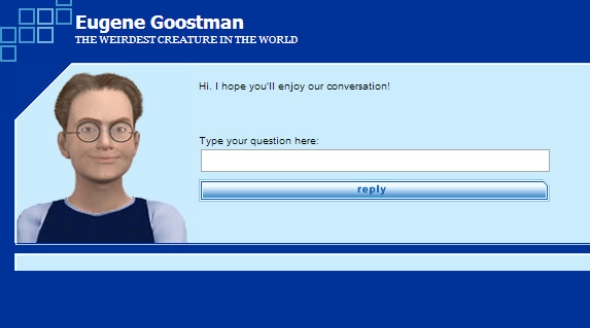
\includegraphics[scale=0.55, clip]{./img/Eugene_Goostman.jpg}
        \caption{チューリングテストを合格したEugeneGoostman\newline(引用:http://www.itmedia.co.jp/news/articles/1807/26/news014.html)}
        \label{fig:チューリングテストを合格したEugeneGoostman}
    \end{center}
\end{screen}
\end{figure}
\newpage
その後,次のAIブームは1950年代後半から1960年代に起きた.
この時代になり初めてAI(Artificial Intelligence,人工知能)という言葉がダートマス会議で用いられた.\\
この会議は1956年に米ニューハンプシャー州のダートマス大学で開催され,コンピュータ研究者たちの研究成果を発表し合う研究発表会である.
この会議の発起人であるジョン・マッカーシー氏がAIという言葉をThe Dartmouth Summer Research Project on Artificial Intelligence\cite{ronbun2}の中で用いた.
また,この会議で初めての人工知能プログラムと言われる“Logic Theorist”と呼ばれる数学原理をコンピュータで証明するデモンストレーションが行われた.
当時のコンピュータはせいぜい四則演算が限界だったので,これは画期的な成果といえた.\\
 他にも,マサチューセッツ工科大学のジョセフ・ワイゼンバウム氏が1966年に作成した単純な自然言語処理プログラム「ELIZA」が発表された.
ただ,ELIZAはそのプログラムはパターン照合を適用しているので,パターンにない会話や曖昧な事柄に対応できない.\\
 また,人工知能の理解は文字列だけにしか及ばず,画像の特徴を自己で判断し抽出することができないシンボルグラウンティング問題が指摘される.
例えば鳩とツノドリの画像を見せ分類するとする時,人間はツノドリのクチバシや足の色などの特徴から分類する.
人工知能はことの時,ツノメドリの特徴として何に着目したらいいのか分からないということが起きるため分類に失敗するという問題がおきた.\\
 1980年代に入り,家庭にコンピュータが普及したことにより第二次ブームが発生した.
「知識」(コンピューターが推論するために必要な様々な情報を,コンピューターが認識できる形で記述したもの)を与えることで人工知能が実用可能な水準に達し,
多数のエキスパートシステムとよばれる,専門分野の知識を取り込んだ上で推論することで,その分野の専門家のように振る舞うプログラムが生み出された.
日本では,政府による「第五世代コンピュータ」と名付けられた大型プロジェクトが推進された.
しかし,当時はコンピューターが必要な情報を自ら収集して蓄積することはできなかったため,必要となる全ての情報について,人がコンピューターにとって理解可能なように内容を記述する必要があり,
世にある膨大な情報全てを,コンピューターが理解できるように記述して用意することは困難なため,実際に活用可能な知識量は特定の領域の情報などに限定する必要があった.
こうした限界から,1995年頃からブームは衰えた.\\
 第二次AIブームでのエキスパートシステムが壁にぶつかった問題として,日常世界には例外処理や矛盾したルールが非常に多く,知識を教え込む作業が非常に困難というのがあった.
これらを解決する手段として「機械学習」や「ディープラーニング」にてコンピュータが自らが学んでいくという手法が第二次AIブームの時代から研究されていたが,実用化するためにはコンピュータの性能が追い付いていなかった.\\
 しかし,2000年代に入り,コンピューターの小型化・性能向上に加えインターネットの普及,クラウドでの膨大なデータ管理が容易となったことで実現可能なレベルとなり,
2006年にはニューラルネットワークの代表的な研究者であるジェフリー・ヒントンらの研究チームが,制限ボルツマンマシンによるオートエンコーダの深層化に成功し,再び注目を集めた.
この際に発表した論文から,これまでの多層ニューラルネットよりもさらに深いネットワーク構造を意味するディープネットワークの用語が定着し,第三次AIブームが沸き起こった.
他にも,2011年にIBMのワトソンが難解な質問と独特の解答方法で知られる人気クイズ番組「ジョパディ!」に出演した.\cite{webpage6}
出演したワトソンが読み込んだ本や映画の脚本,百科事典などは合計100万冊にものぼり,公平を期すため,インターネットには接続しておらず,読み込んだデータのみでの勝負となり,歴代チャンピオン2人に勝利した.\\
 2012年にはGoogleが発表した機械学習の論文では,事前に猫をネットワークに教えたわけでもなく,猫のラベル付けした画像を与えたわけではない人工知能を発表した.\cite{ronbun3}
このときまで,機械学習のほとんどは,ラベル付きデータの量に依存していた.
この論文により,機械がラベルのない生データでも処理することができ,そしておそらく,人間が予備知識を持たないデータですら処理できることが示された.
\begin{figure}[!ht]
    \begin{screen}
    \begin{center}
        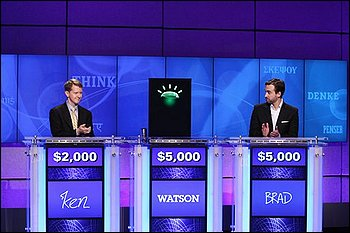
\includegraphics[scale=1.1, clip]{./img/Watson.jpg}
        \caption{クイズ番組に出演するWatson\newline(http://www.swift-web.org/cp-bin/blogn/index.php?e=1023)}
        \label{fig:クイズ番組に出演するWatson}
    \end{center}
\end{screen}
\end{figure}\\
\newpage
\subsection{現在のAI}
2014年にはAmazon.comからスマートスピーカと呼ばれる対話型の音声操作に対応したAIアシスタント機能を持つスピーカーであるAmazon Echoが発売され,その後GoogleやAmazon,IBMによって様々なスマートスピーカーが商品化された.
現在ではスマートフォンにもSiriというAIが搭載されるなどその存在は非常に身近になっており,その種類も非常に多岐にわたる.
\begin{figure}[!ht]
    \begin{screen}
    \begin{center}
        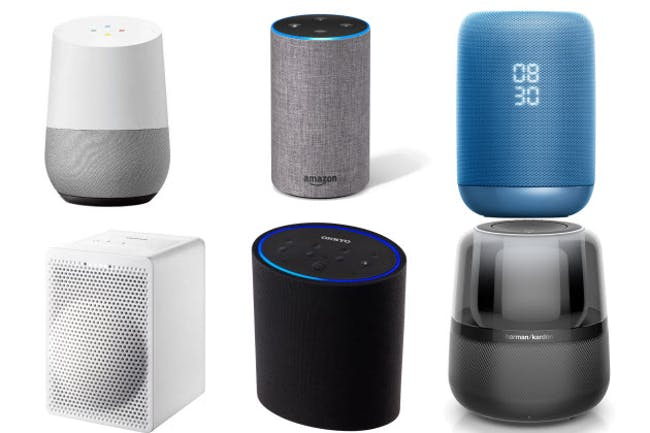
\includegraphics[scale=0.6, clip]{./img/smartspeaker_list.jpg}
        \caption{多種多様なスマートスピーカー}
        \label{fig:多種多様なスマートスピーカー}
    \end{center}
\end{screen}
\end{figure}\\
囲碁や将棋,チェスなどの競技においても,プロにAIが勝利するなど(\ref{fig:電王戦の様子})その精度は以前より高いが,そのAIは一つの競技でしか使用できない特化型人工知能(AGI)であった.
しかし,英DeepMindが発表したAlphaZeroという様々なボードゲームに対応できる汎用性を持ったAIが発表され,以降,汎用人工知能(GAI)の成長も著しい.\\
 自然言語処理を用いた芸術の分野では,2012年にスタートした人工知能を使って小説を生成するプロジェクトが「星新一賞」の第一審査を通過した.\cite{webpage2}
また,芸術の分野に関してもAIが作成した肖像画が米競売大手クリスティーズのオークションで43万2500ドル(約4900万円)で落札されたり,AIを用いて新しい楽曲を作るものが出回っていたりと,成長が著しい.\cite{webpage3}\\
\newpage
\begin{figure}[!ht]
    \begin{screen}
    \begin{center}
        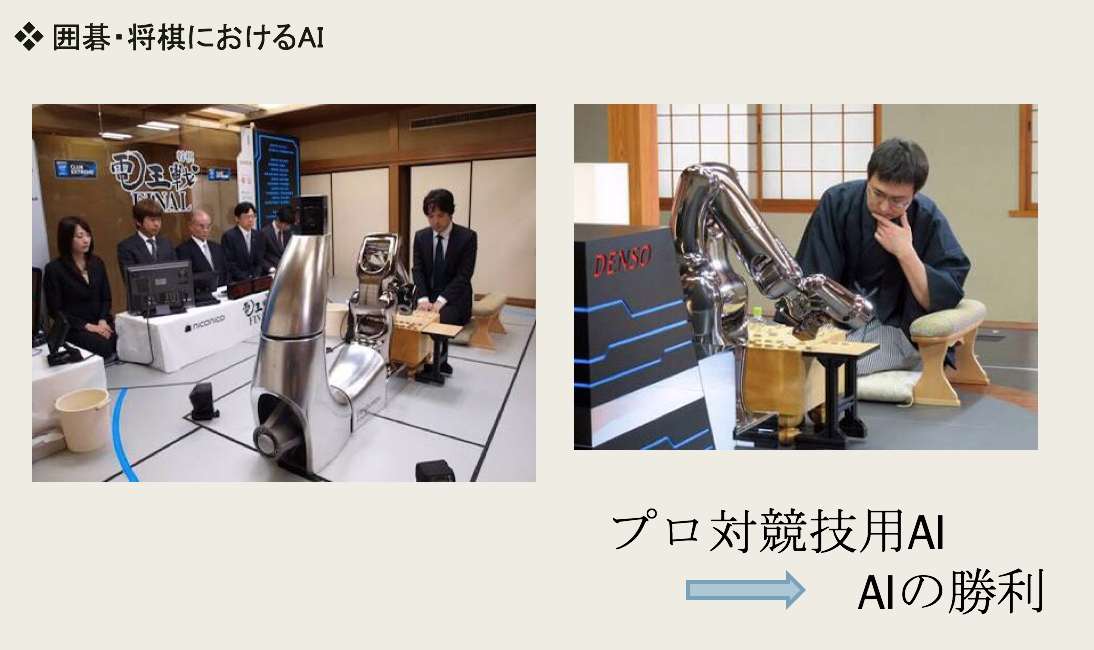
\includegraphics[scale=0.7, clip]{./img/igo1.png}
        \caption{電王戦の様子}
        \label{fig:電王戦の様子}
    \end{center}
\end{screen}
\end{figure}\\
\newpage
\section{AIを用いた楽曲作成}
作曲の流れはその構成によって階層化されており,比較的自動化が容易とされている.音楽を構成する3要素はスケール(調)とコード(和音)とメロディ(旋律)とされており,スケールが決まればその構成音に合わせてコードも決まる.コード進行は一定のルールがあり,これまでの曲の中で良い進行とされるパターンは数多く蓄積されている.コードは曲のムードを大きく左右し、
人間のその時の感情、感じ方に非常に影響を与えると言われている.メロディも同様にコードの構成音を元にすれば大きく外れることはないが,単調になってしまう傾向があるので,多少のランダムさが必要とされている要素である.コードに対して大きく外さない範囲で変動させれば単調になるのを防ぐこともできる.
%MIDIである必要性:なぜこれを使うのか波形でない理由
\subsection{MIDI}
音楽データには大きく分けて二つある.一つ目はオーディオデータといい波形の情報を記録する形式であり,二つ目がMIDIである.\\
 MIDI(Musical Instrument Digital Interface)は,日本のMIDI規格協議会(JMSC,現在の社団法人音楽電子事業協会)と国際団体のMIDI Manufacturers Association (MMA) により策定された,電子楽器の演奏データを機器間でデジタル転送するための世界共通規格で,物理的な送受信回路・インタフェース,通信プロトコル,ファイルフォーマットなど複数の規定からなる.MIDIは単なるデータであり、マシン同士が通信につかう一連の指令である.\\
 本研究で用いるAIはこのMIDIファイルの情報を元に学習をする.これはMIDIは実際の音ではなく音楽の演奏情報(音を出す,音の高さ,長さなど)のデータであり,各パートごとにトラックが分かれているため,すべての音が混合されているオーディオデータと違いMIDIの方が特徴をつかみやすいからである.
また入出力の際もこの規格を用いる.\\
 MIDIには以下の情報が含まれている.
\begin{figure}[!ht]
    \begin{screen}
・鍵盤のオンとオフ: 鍵盤がいつ押されたのか/離されたのか\\
・演奏した音程 ベロシティー: どれだけの早さと強さで打鍵されたか\\
・アフタータッチ: どのくらいの強さで鍵盤が押さえられているか\\
・テンポ(もしくはBPM)\\
・パン\\
・モジュレーション\\
・音量\\
    \end{screen}
\end{figure}\\
 音の高さは最も低い音を0、最も高い音を127で半音刻みで割り当てられている.楽曲制作の際に音程を指定する場合は図\ref{fig:MIDIと音階}の数値を指定する.
\begin{figure}[h]
    \begin{screen}
    \begin{center}
        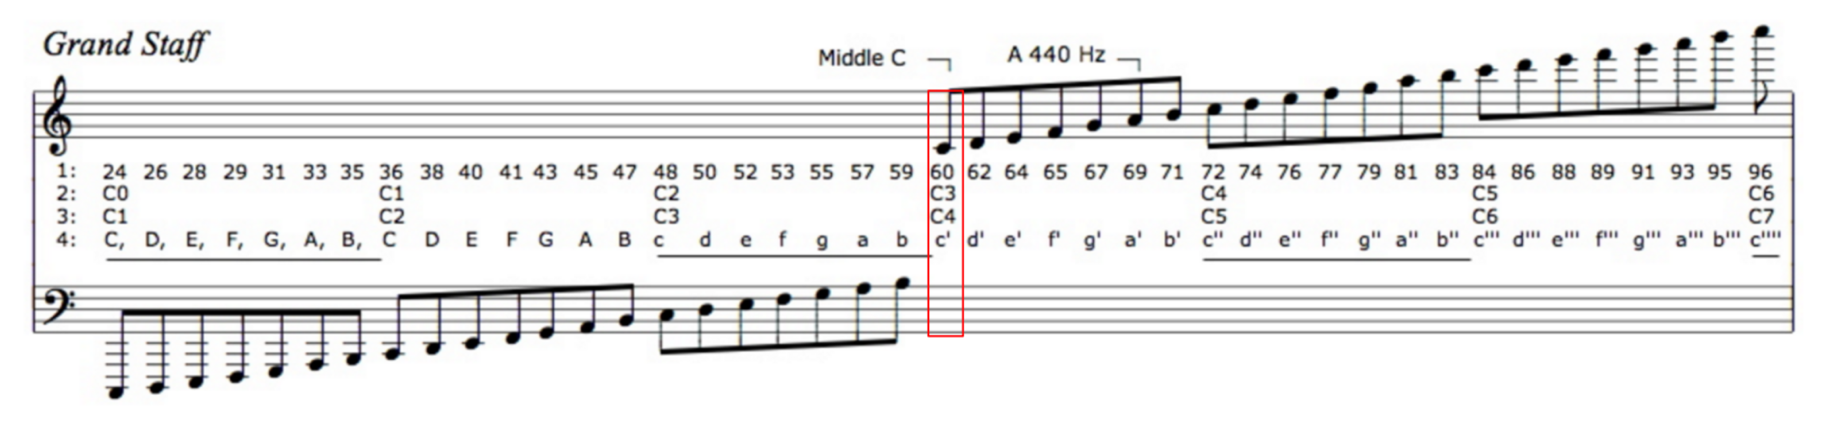
\includegraphics[scale=0.45,clip]{./img/midi2.png}
        \caption{MIDIと音階}
        \label{fig:MIDIと音階}
    \end{center}
    \end{screen}
\end{figure}
%AIを用いた楽曲サービスについて述べてその中でなぜMagendaを選ぶのかを述べる
\newpage
\subsection{Magenta}
本研究で使用するMagentaは音楽などをTensorFlowを使って機械学習するライブラリであり,Google BrainがGitHub上に公開されているOSSである.これを図\ref{fig:GitHub上に公開されているMagenta}に示す.\\
 Magentaではまず学習させたい音楽のMIDIデータをNoteSequence(magentaが扱うファイル形式)とよばれるデータフォーマットに変更する.それを学習用データセットと評価用データセットに変換したあと学習を行う.
このとき,一度に学習させるデータの数,学習を行う回数,ノード数を設定する.これをパッケージ化し,MIDIファイルとして新たに楽曲を生成するという流れである.これを図\ref{fig:magentaによるMIDI音楽データ生成までのプロセス}に示す.
\begin{figure}[h]
    \begin{screen}
    \begin{center}
        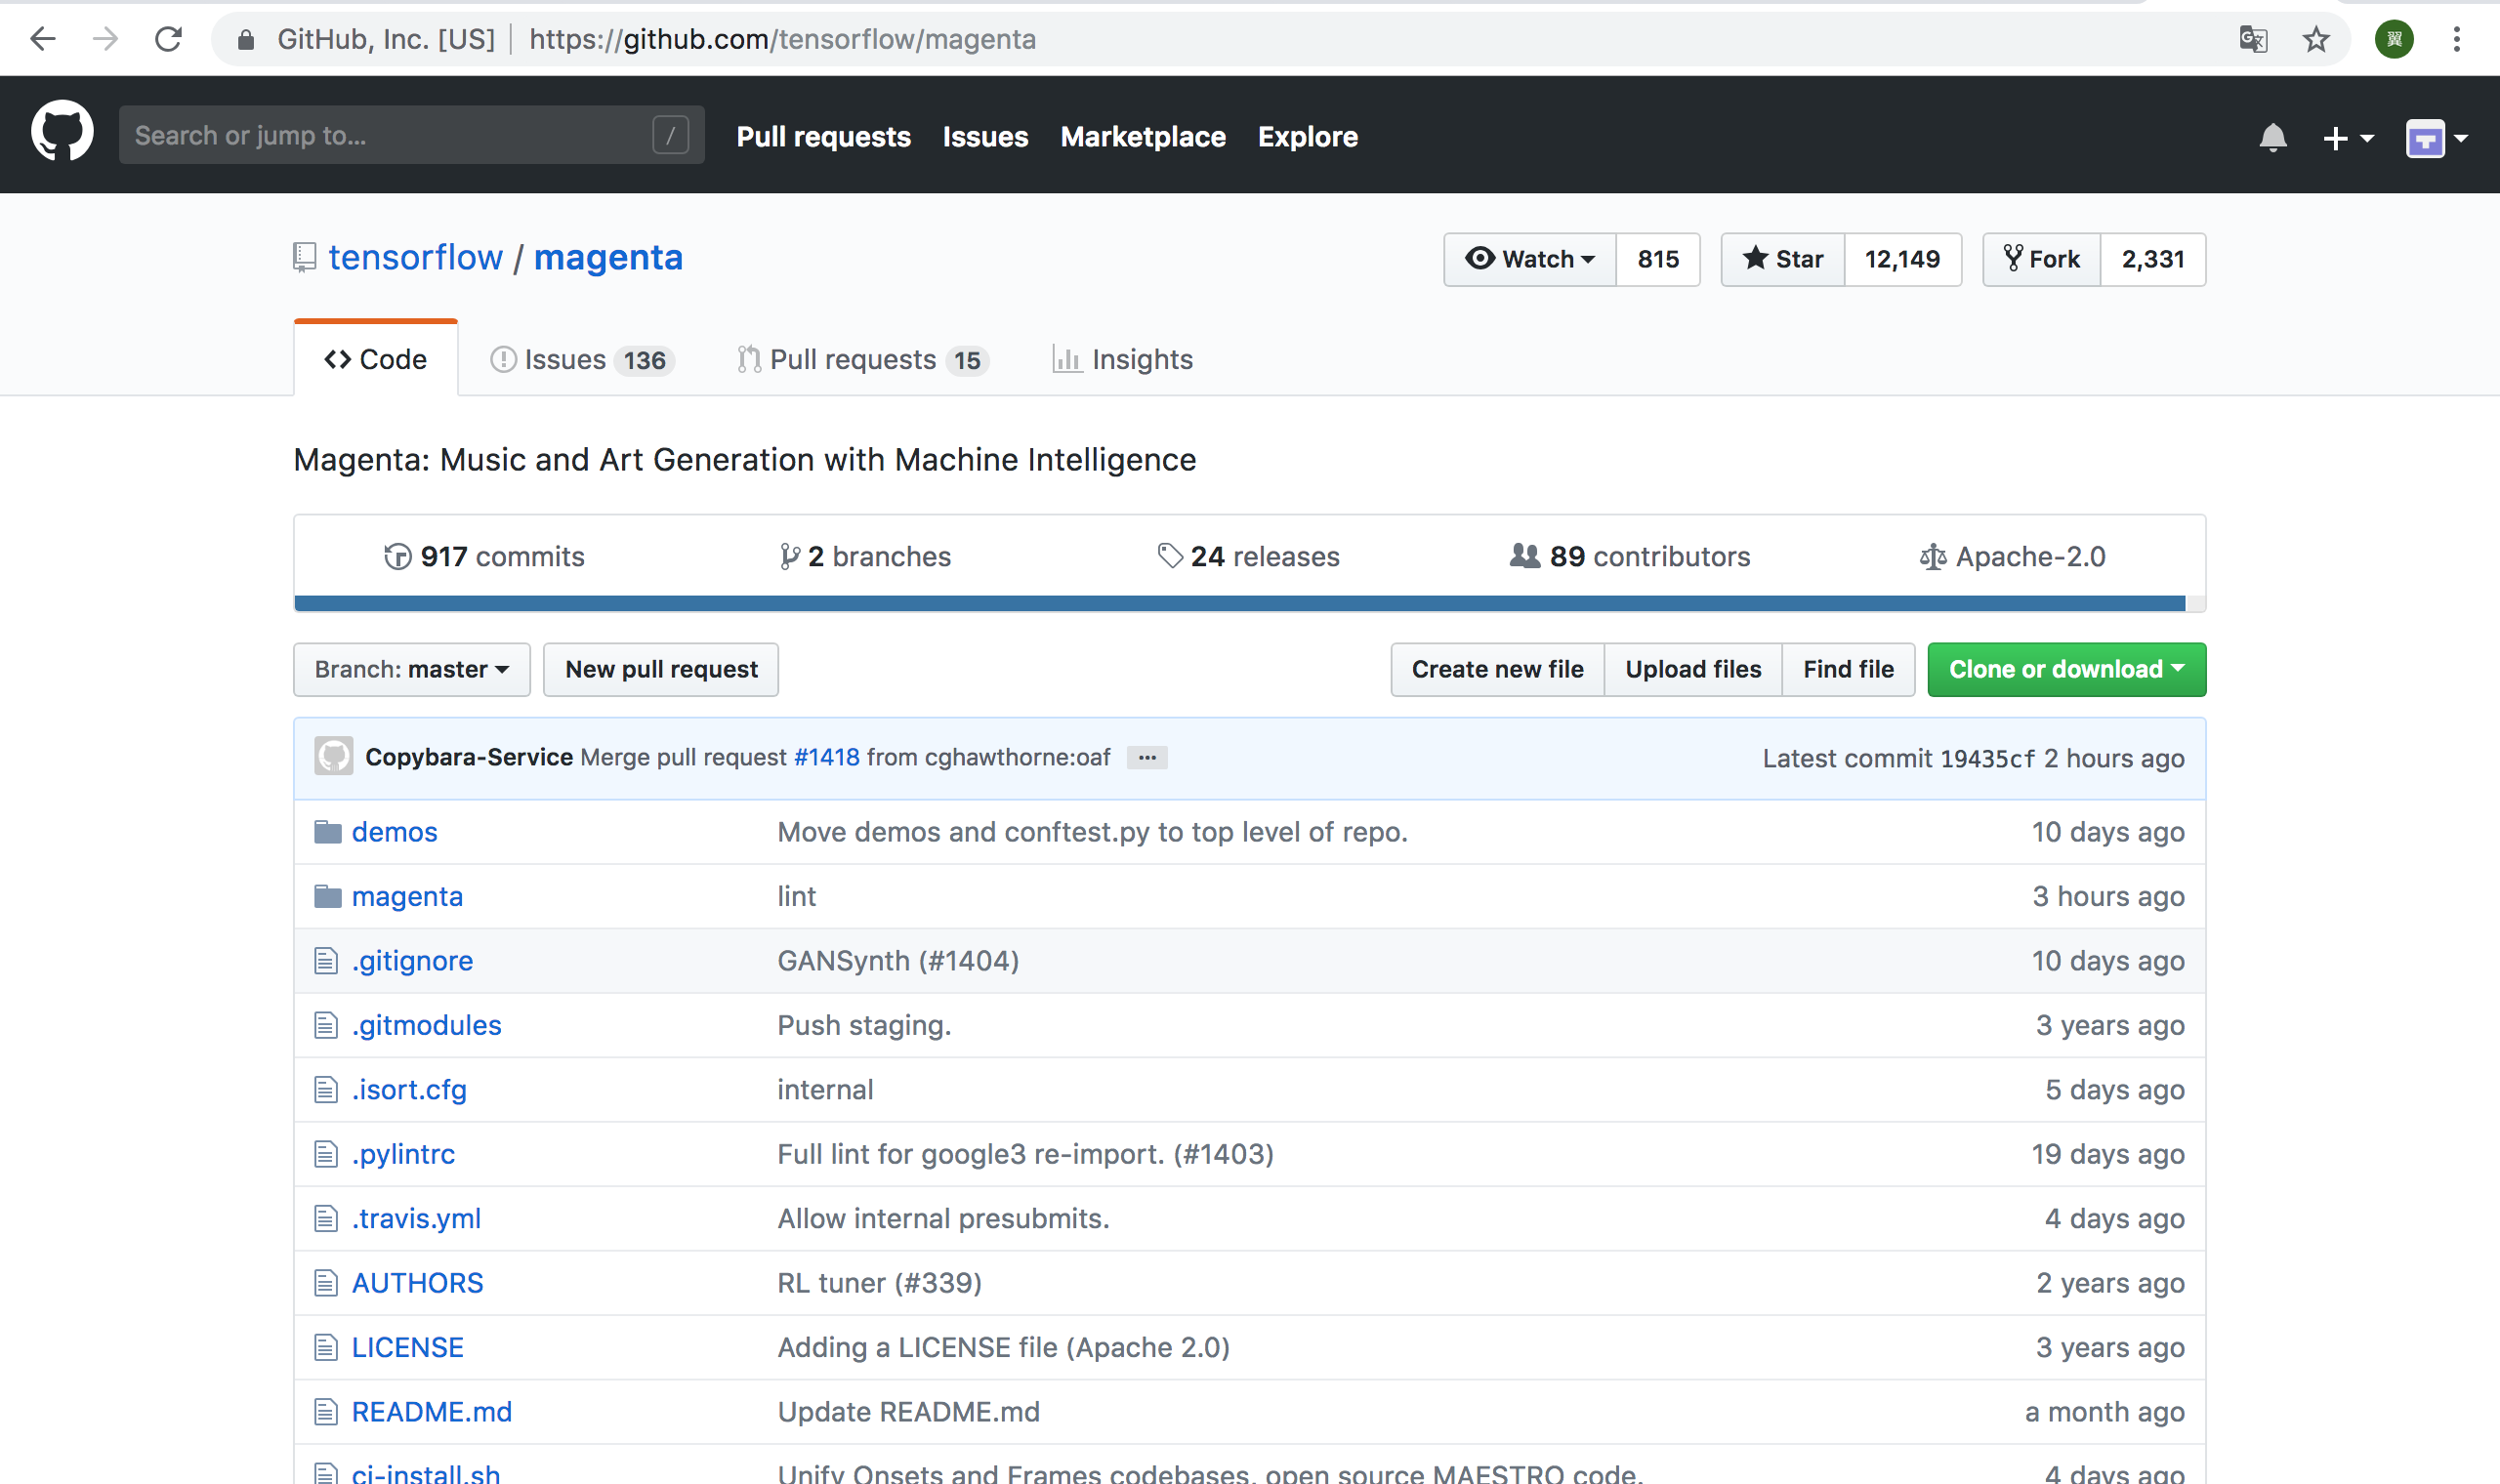
\includegraphics[scale=0.3, clip]{./img/magentagithub.png}
        \caption{GitHub上に公開されているMagenta}
        \label{fig:GitHub上に公開されているMagenta}
    \end{center}
    \end{screen}
\end{figure}
\newpage
\begin{figure}[h]
    \begin{screen}
    \begin{center}
        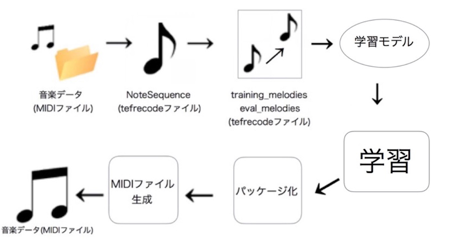
\includegraphics[scale=1.7, clip]{./img/magenta_usestep.png}
        \caption{magentaによるMIDI音楽データ生成までのプロセス}
        \label{fig:magentaによるMIDI音楽データ生成までのプロセス}
    \end{center}
    \end{screen}
\end{figure}
 なお,インプットデータはone-hot Vectorで図\ref{fig:インプットデータの仕組み}のようになっている.
\begin{figure}[h]
    \begin{screen}
    \begin{center}
        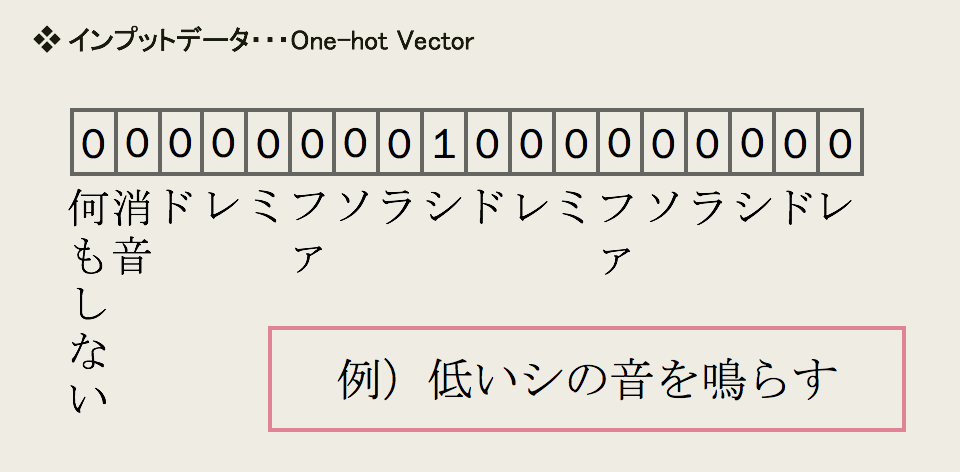
\includegraphics[scale=0.85,clip]{./img/midi1.png}
        \caption{インプットデータの仕組み}
        \label{fig:インプットデータの仕組み}
    \end{center}
    \end{screen}
\end{figure}
\subsection{リカレントニューラルネットワーク(RNN)}
本研究で用いるMagentaのモデルはRNN(Recurrent Neural Network)を取り入れたものである.
RNNは、ある層の出力がもう一度その層へ入力される回帰結合を持つニューラルネットワークである.
このような結合を持つことで、ニューラルネットは過去の情報を保持することができるようになる.
\newpage
\section{機械学習に適した開発環境について}
Tensolflowのランタイムとして以下のシステムがサポートされている.\cite{webpage8}
\begin{enumerate}
    \renewcommand{\labelenumi}{(\arabic{enumi})}
    \item Ubuntu 16.04以降
    \item macOS 10.12.6(Sierra)以降(GPUサポートなし)
    \item Windows7 以降
    \item Raspbian 9.0以降
\end{enumerate}
 また,GPUを用いて学習を行う時にはtensolflow-gpuというパッケージが必要となり,導入には以下のドライバやライブラリが必要である.\cite{webpage7}
\begin{enumerate}
    \renewcommand{\labelenumi}{(\arabic{enumi})}
    \item CUDA Toolkit (tensolflowはCUDA9.0をサポート)
    \item CUPTI (CUDA Toolkitに付随)
    \item NVIDEAGPUドライバ(CUDA9.0には384.x以上が必要)
    \item cuDNN SDK
\end{enumerate}
 Windows10の環境ではリリースされているCUDAのバージョンは10のみであり,Tensolflowのサポートを外れてしまう.
そのため,CUDAv9がインストール可能なUbuntuを用いることとし,システムの開発環境を表\ref{tab:開発環境}に示す.
\begin{table}[h]
\begin{center}
\caption{開発環境}
\label{tab:開発環境}
\begin{tabular}{|c|p{20zw}|}
\hline
    OS & Ubuntu 16.04 LTS\\
    \hline
    CPU & Intel Core i3 8100\\
    \hline
    メモリ & 8GB\\
    \hline
    GPU & GeForce GTX 1060\\
    \hline
    CUDA & CUDA(9),cuDNN(7.4.2)\\
    \hline
    ライブラリ & TensorFlow(1.12.0),magenta(0.5.0)\\
    \hline
\end{tabular}
\end{center}
\end{table}\\
\newpage
\subsection{CUDA}
CUDAは,NVIDIAが開発しているGPU上でプログラミングをするためのソフトウェアプラットフォームである.
含まれるものとしては,CUDAを実行形式に変えるコンパイラや,それをサポートするSDK,ライブラリ,デバッグツール群である.
CUDAを導入することによって,プログラムを複数のプロセッサで動かすだけでなく,無駄なく並列化することができる.
導入に成功すれば,以下のように学習時にGPUの名前やメモリの状態が表示され,学習に使用される.
\begin{lstlisting}[basicstyle=\ttfamily\footnotesize,frame=single]
INFO:tensorflow:Graph was finalized.
2019-01-31 16:19:01.831071: 
I tensorflow/core/platform/cpu_feature_guard.cc:141]
    Your CPU supports instructions that this TensorFlow
    binary was not compiled to use: AVX2
2019-01-31 16:19:02.120562: 
I tensorflow/core/common_runtime/gpu/gpu_device.cc:1432]
    Found device 0 with properties:
name: GeForce GTX 1060 6GB major: 6 
minor: 1 memoryClockRate(GHz): 1.759
pciBusID: 0000:01:00.0
totalMemory: 6.00GiB freeMemory: 4.96GiB
2019-01-31 16:19:02.131909:
    I tensorflow/core/common_runtime/gpu/gpu_device.cc:1511] 
Adding visible gpu devices: 0
2019-01-31 16:19:03.556213:
    I tensorflow/core/common_runtime/gpu/gpu_device.cc:982]
Device interconnect StreamExecutor with strength 1
    edge matrix:
2019-01-31 16:19:03.562443:
    I tensorflow/core/common_runtime/gpu/gpu_device.cc:988]
        0
2019-01-31 16:19:03.566344:
    I tensorflow/core/common_runtime/gpu/gpu_device.cc:1001]
    0:   N
2019-01-31 16:19:03.570191:
    I tensorflow/core/common_runtime/gpu/gpu_device.cc:1115]
    Created TensorFlow device
    (/job:localhost/replica:0/task:0/device:GPU:0 with 4714MB memory)
-> physical GPU 
(device: 0, name: GeForce GTX 1060 6GB,
 pci bus id: 0000:01:00.0, compute capability: 6.1)
INFO:tensorflow:Restoring parameters from
    C:\Users\matsumoto\magenta
    \melody_rnn\logdir\run1\train\model.ckpt-170
INFO:tensorflow:Running local_init_op.
INFO:tensorflow:Done running local_init_op.
WARNING:tensorflow:From 
C:\Users\matsumoto\AppData\Local\Programs\Python\Python36\lib
\site-packages\tensorflow\python\training\monitored_session.py:804:
    start_queue_runners 
    (from tensorflow.python.training.queue_runner_impl)
     is deprecated and will be removed in a future version.
Instructions for updating:
To construct input pipelines, use the `tf.data` module.
\end{lstlisting}
